\section{A result that can be inspected and changed}
\label{section:the-backend-objects-authority-and-revision}

A memory answer needs a route back to its sources. A research result needs that route too, together with a record of the assumptions, calculations and judgements that make it usable. Someone else must be able to inspect it, change its inputs and understand what must be reconsidered. The Writing App is an integrated research environment built around that continuity. It keeps the material, the claims made about it, the work performed on it and the decisions that accept it connected. The manuscript is one view of that research state. Calculations, source passages and review are other views, with tools for moving between them.

Take the gap-aware quantum example. A calculation reports that a gap-aware enlargement sharply reduces the energy error in a specified model and candidate pool. A claim states what that comparison supports. A figure displays it, and a paragraph explains why the energy denominator helped. A reviewer may ask whether the same selection rule works on another Hamiltonian. That question needs the model, pool, selection rule and original result, together with a way to add the next calculation without losing the first.

\subsection{An object carries its grounds}
The system gives each of these objects an identity and an interface. Its detailed material may be a mathematical statement, a table, code, a source passage or a reference to a larger file. Around that material sit a readable summary, typed relationships, revision information and the operations currently allowed. We call this organising pattern a \emph{conceptric envelope}: a unit of knowledge that carries enough context to be inspected and safely used elsewhere.

Figure~\ref{fig:dd-conceptric-envelope} follows the claim in the quantum example. Its exterior says what the result concerns and how to inspect it. Inside are the statement, assumptions and exact grounds. The relationships say that a source supports a method, a calculation tests a configuration, and a figure or paragraph uses the resulting claim. Giving these relationships types makes a practical difference. A source citation supplies documentary support, while a logical premise supplies something the argument requires. A chapter contains a paragraph, while a review task depends on the version it inspected.

Two kinds of digest help here. A readable digest tells another reader or task what the object means. A content digest or revision identifies which version was used. The first makes a large collection navigable, while the second makes a later comparison exact. The app exposes these through the existing claim, source, result and Work interfaces, with each kind of object retaining the details appropriate to its job.

\begin{figure}[htbp]
\centering
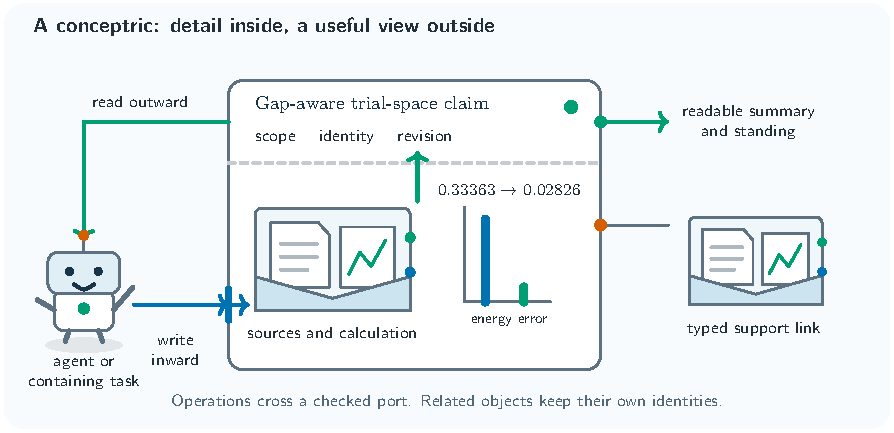
\includegraphics[width=\linewidth]{figures/robot-run-c4d4b3872a904ec0.result/dd-conceptric-envelope.pdf}
\caption{A claim with a readable exterior. The gap-aware comparison retains its model, candidate pool and source/result links, while the containing task receives a concise account of what it can use. The action interface admits changes against the current version. Blue marks the object and its operations, teal the outward flow of observations.}
\label{fig:dd-conceptric-envelope}
\end{figure}

The direction of information is important. Here \emph{inside} means an object's detailed material and local state, and \emph{outside} means its interface and the task that contains or uses it. \emph{Reading goes in to out}: observations of the inner material become the summary or selected detail exposed to that task. A request to open a source points inward, but the information returned from it flows outward. \emph{Writing goes out to in}: an outer intention, such as revising the energy claim, is narrowed to an allowed operation on a particular inner object. Its outcome then becomes visible outside again.

This arrangement gives a task control over its level of detail. A comparison of methods may need a result summary and its conditions. Checking one number may need the precise configuration and table row. Editing a caption needs the figure's data and the current words. The system supplies bounded observations for those different purposes and provides explicit routes to further detail. Semantic selection still matters: the author or agent must ask for the material the inference needs.

\subsection{An authorised change}
The \emph{harness} is the software around the model that prepares its context, exposes tools and routes their requests. It starts with the selected project, the author's question, the relevant objects and the session's role. A working author session and an independent reviewer have different available operations. A child calculation also has a declared task and a place to return its result. These boundaries make responsibility visible before an action is taken.

Suppose the AI wants to link the new calculation to the energy claim. It submits a structured request identifying both objects and the revisions it has inspected. The gateway checks the operation, the role and the project scope. The request then reaches the \emph{owner}, the application component responsible for that kind of change. The owner checks the relevant current identities and records the admitted transition. Source editing adds its own checks on the selected manuscript, exact original passage and proposed replacement. Figure~\ref{fig:dd-ai-tool-harness} shows this route.

\begin{figure}[htbp]
\centering
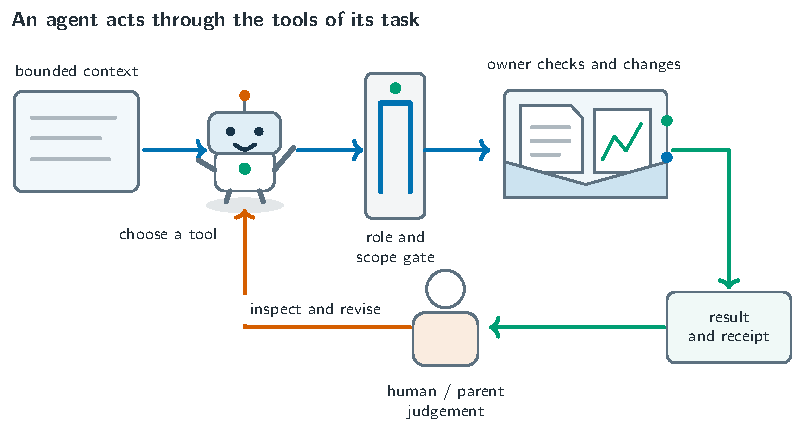
\includegraphics[width=\linewidth]{figures/robot-run-c4d4b3872a904ec0.result/dd-ai-tool-harness.pdf}
\caption{From a model request to an inspectable result. The harness supplies task context and checks permission. The owning operation checks the current basis and records the change. The human and parent task can inspect the same outcome, judge its interpretation and request a revision. The loop keeps the proposal, action and acceptance connected.}
\label{fig:dd-ai-tool-harness}
\end{figure}

The return explains what happened and where to inspect it. For a numerical producer, that includes its inputs, execution outcome and output. For a source change, it includes the affected passage and recorded revision. If a write lands but a later recording step is interrupted, the recovery mechanism is designed to use the retained source effect to distinguish a committed edit from a pending record. It can then finish the record without replaying the source edit.\footnote{The linked implementation account identifies source-inspected recovery branches. The successful figure application described below is not an interrupted-operation test. This account does not display an executed recovery trace.}

Scientific acceptance enters at a different point in the same route. A human or designated model reviewer judges whether the evidence supports the stated interpretation. The literature tool records that judgement alongside the observed passage and the claim version. Numerical checks test a declared calculation. Formal checks test an encoded proposition and its assumptions. The parent task brings those contributions together and records what it accepts. Each participant can inspect the basis of the decision and challenge the relevant step.

The implementation keeps a passage observation separate from the judgement that it supports a claim. A current file identifies the material used. A support judgement says what someone concluded from it. A containing task's acceptance records which contribution it admitted. None substitutes for the others.

\subsection{What the change affects}
Now change the candidate pool used by the quantum calculation. The original result still describes its original pool. The new input gives the next calculation a different basis, and any explanation that intends to use the new result needs attention. A paragraph's wording may remain byte-for-byte unchanged while its supporting comparison has moved. This is why the system tracks a content revision separately from the currentness of its grounds.

Work records make the consequence actionable. A task stores its objective, current standing, declared prerequisites and completion evidence. Acceptance retains the exact prerequisite completions and evidence it consumed. When one of those changes, the current observation can mark that acceptance stale and identify the affected input. A new run, revised interpretation or fresh review can then restore the local chain. The scope of this propagation is the declared dependency graph. It gives the system a precise way to ask what needs reconsidering, while people and reviewers decide how the scientific account should change.

The human interface exposes the same state through manuscript, research, reference, logical-structure and Work views. The AI enters through tools that reach the same owners. A reader can open the claim, follow its result or source, inspect the proposed change and see its outcome. For repository inspection, \nolinkurl{docs/writing-source-map.md} is the entry point, with the transaction in \nolinkurl{src/laplace/manuscript/source_application.py}, context admission in \nolinkurl{src/laplace/writing/turn_admission.py}, and task acceptance in \nolinkurl{src/laplace/work/project_work.py}.

The hierarchy figure in this account followed that route. A supervised calculation produced the stability curves and checked their boundary against the linearised dynamics. We interpreted the result, bound it to the feedback claim, and revised the explanation and figure placement against the current source. The editor preserved the preceding text, recorded the application and rebuilt the PDF. A reader can consequently move from the displayed boundary back to the model and calculation, or forward from the claim to the passage that uses it.

The open-systems discussion gives a useful design comparison. A scientific object's meaning depends on its context: a Hamiltonian convention, candidate pool or source version can change what its conclusion supports. Eigen retains those consequential relationships at the object's boundary, while exposing only the detail needed by the current task. When a surrounding assumption changes, the relevant consumer must be reconsidered. The boundary retains the dependencies that make a local operation safe to compose with the rest of the work.

The connection to the earlier theory is now concrete. A useful representation keeps the distinctions required by an operation and exposes the cost of losing them. For this software, those distinctions include the material, its interpretation, the authority to change it and the evidence on which a decision rests. Preserving them lets a small local operation participate in a larger research process. The same boundary can then be repeated at the level of a calculation, a manuscript section or an entire project.
